\begin{figure}[t]
\begin{center}
	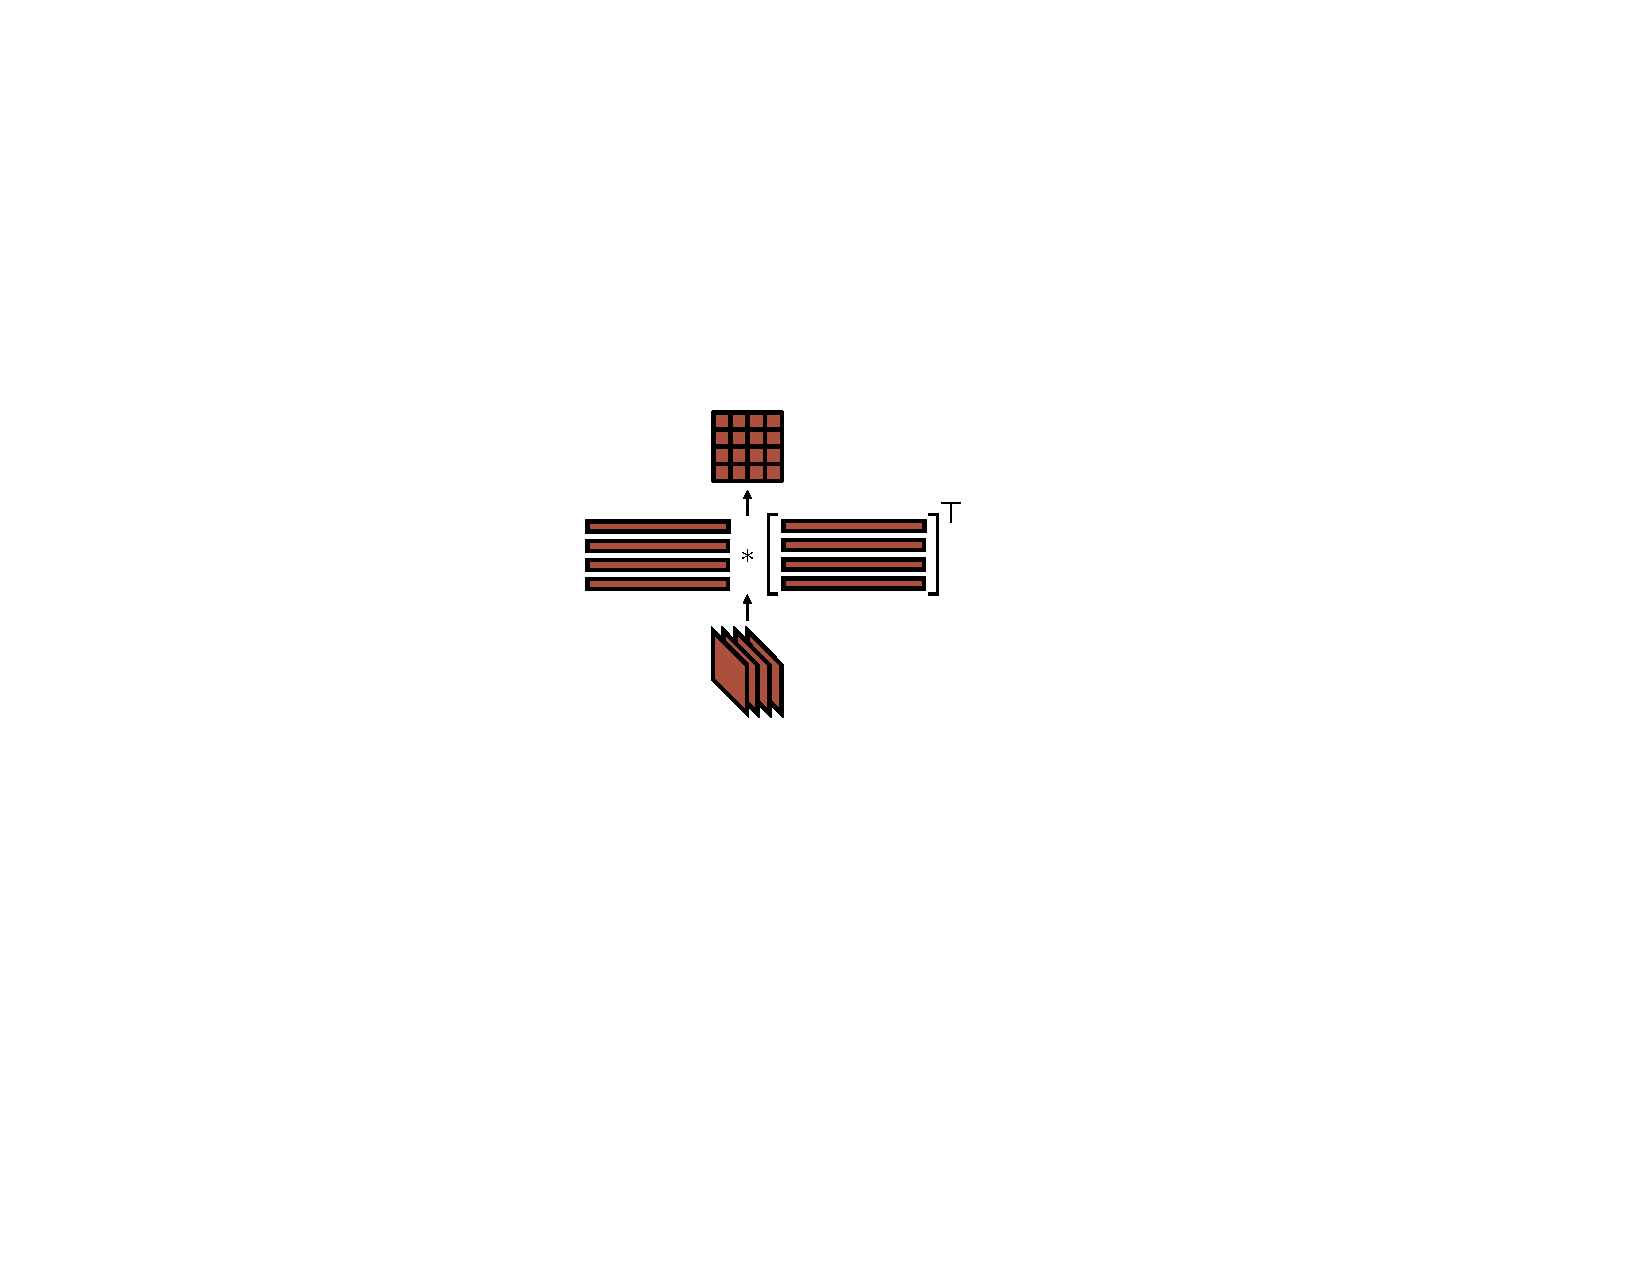
\epsfig{file=gram_matrix.pdf, width = 0.6 \textwidth}\\
	\caption[Computing the Gram matrix from activation maps]{Computing the Gram matrix from the activation maps of a layer. Activation maps are first reshaped to row vectors, then the Gram matrix is realized by computing the inner product between the row-vectorized activation maps and their transpose.}
	\vspace{-0.65cm}
	\label{fig:gram_matrix}
\end{center}
\end{figure}